\chapter{Sistema en un Chip (SoC)}

En esta secci�n estudiaremos la arquitectura b�sica de un SoC moderno, componentes, funcionamiento, programaci�n y operaci�n. Como se mencion� anteriormente, la tendencia actual de la industria de los semiconductores es integrar en un solo dispositivo las funcionalidades necesarias para la implementaci�n de dispositivos digitales modernos. Esto es posibe gracias a los grandes avances en las t�cnicas de fabricaci�n de circuitos integrados y a la demanda de nuevas caracter�sticas exigidas por los fabricantes de dispositivos digitales de consumo masivo como tel�fonos celulares, PDAs, consolas de juegos y reproductores multimedia. Para utilizar estos avances tecnol�gicos es necesario conocer su arquitectura, principio de funcionamiento, programaci�n e implementaci�n, para esto, se estudiar�n dos proyectos abiertos que implementan un SoC en un PLD utilizando lenguaje de descripci�n de hardware y herramientas GNU; proporcionan el c�digo fuente, lo que permite un estudio profundo de su arquitectura. El proyecto \textit{Plasma} \cite{SR08} y el proyecto Mico32\cite{LSC08}.


\section{Arquitectura}

Un SoC, integra un conjunto de perif�ricos, memorias y una o varias unidades de procesamiento (CPUs) en un solo chip, lo cual facilita el desarrollo de aplicaciones. Comercialmente encontramos una gran variedad de configuraciones CPU - perif�ricos, dependiendo de la aplicaci�n; dentro de los m�s comunes se encuentran: controladores de memorias externas (NOR, NAND, SDRAM, DDR), puertos de comunicaci�n (I2C, SPI), puerto de depuraci�n (UART), timers, reloj de tiempo real, codecs de audio, controladores de LCD, controladores de red, controlador de puerto USB host, controlador para sensores de im�genes, etc. La figura \ref{min_soc_arch} muestra una arquitectura de un SoC sencillo con los componentes necesarios para implementar tareas simples.


\begin{figure}
  \begin{center} 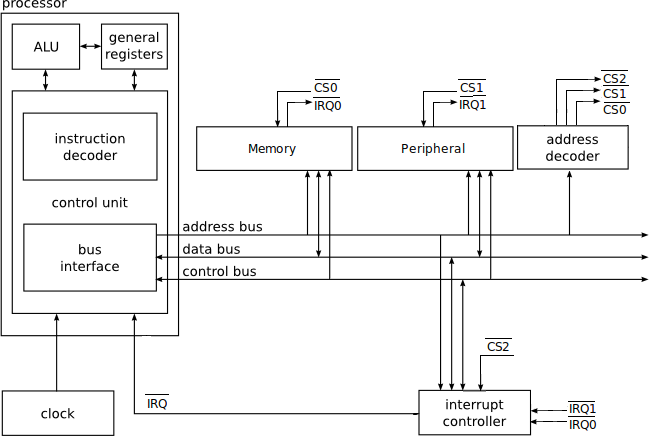
\includegraphics[scale=.6]{./images/Computer-simple} \end{center}
  \caption{Arquitectura m�nima de un SoC}\label{min_soc_arch}
\end{figure}

\subsubsection{Unidad de Procesamiento Central (CPU)}

La unidad de procesamiento central (CPU), como su nombre lo indica, est� encargada de centralizar las tareas del sistema coordinando las acciones de los perif�ricos. Puede ser vista como una m�quina de estados programable que controla un camino de datos compuesto por bloques aritm�ticos, l�gicos y un banco de registros. Cada CPU es capaz de realizar una serie de operaciones sobre variables almacenadas en el banco de registros, estas operaciones reciben el nombre de \textit{conjunto de instrucciones}. El programador utiliza estas instrucciones para hacer que la CPU realice una funci�n espec�fica, indicandole paso a paso donde debe leer la informaci�n, como procesarla y como entregar el resultado. A Esta funci�n se le conoce con el nombre de programa o tarea Software.


\subsubsection{Perif�ricos}
Los perif�ricos proporcionan la comunicaci�n con el exterior, permiten el ingreso, almacenamiento y procesamiento de la informaci�n


